% Options for packages loaded elsewhere
\PassOptionsToPackage{unicode}{hyperref}
\PassOptionsToPackage{hyphens}{url}
\PassOptionsToPackage{dvipsnames,svgnames,x11names}{xcolor}
%
\documentclass[
  12pt]{article}

\usepackage{amsmath,amssymb}
\usepackage{iftex}
\ifPDFTeX
  \usepackage[T1]{fontenc}
  \usepackage[utf8]{inputenc}
  \usepackage{textcomp} % provide euro and other symbols
\else % if luatex or xetex
  \usepackage{unicode-math}
  \defaultfontfeatures{Scale=MatchLowercase}
  \defaultfontfeatures[\rmfamily]{Ligatures=TeX,Scale=1}
\fi
\usepackage{lmodern}
\ifPDFTeX\else  
    % xetex/luatex font selection
\fi
% Use upquote if available, for straight quotes in verbatim environments
\IfFileExists{upquote.sty}{\usepackage{upquote}}{}
\IfFileExists{microtype.sty}{% use microtype if available
  \usepackage[]{microtype}
  \UseMicrotypeSet[protrusion]{basicmath} % disable protrusion for tt fonts
}{}
\makeatletter
\@ifundefined{KOMAClassName}{% if non-KOMA class
  \IfFileExists{parskip.sty}{%
    \usepackage{parskip}
  }{% else
    \setlength{\parindent}{0pt}
    \setlength{\parskip}{6pt plus 2pt minus 1pt}}
}{% if KOMA class
  \KOMAoptions{parskip=half}}
\makeatother
\usepackage{xcolor}
\setlength{\emergencystretch}{3em} % prevent overfull lines
\setcounter{secnumdepth}{5}
% Make \paragraph and \subparagraph free-standing
\ifx\paragraph\undefined\else
  \let\oldparagraph\paragraph
  \renewcommand{\paragraph}[1]{\oldparagraph{#1}\mbox{}}
\fi
\ifx\subparagraph\undefined\else
  \let\oldsubparagraph\subparagraph
  \renewcommand{\subparagraph}[1]{\oldsubparagraph{#1}\mbox{}}
\fi


\providecommand{\tightlist}{%
  \setlength{\itemsep}{0pt}\setlength{\parskip}{0pt}}\usepackage{longtable,booktabs,array}
\usepackage{calc} % for calculating minipage widths
% Correct order of tables after \paragraph or \subparagraph
\usepackage{etoolbox}
\makeatletter
\patchcmd\longtable{\par}{\if@noskipsec\mbox{}\fi\par}{}{}
\makeatother
% Allow footnotes in longtable head/foot
\IfFileExists{footnotehyper.sty}{\usepackage{footnotehyper}}{\usepackage{footnote}}
\makesavenoteenv{longtable}
\usepackage{graphicx}
\makeatletter
\def\maxwidth{\ifdim\Gin@nat@width>\linewidth\linewidth\else\Gin@nat@width\fi}
\def\maxheight{\ifdim\Gin@nat@height>\textheight\textheight\else\Gin@nat@height\fi}
\makeatother
% Scale images if necessary, so that they will not overflow the page
% margins by default, and it is still possible to overwrite the defaults
% using explicit options in \includegraphics[width, height, ...]{}
\setkeys{Gin}{width=\maxwidth,height=\maxheight,keepaspectratio}
% Set default figure placement to htbp
\makeatletter
\def\fps@figure{htbp}
\makeatother

\addtolength{\oddsidemargin}{-.5in}%
\addtolength{\evensidemargin}{-1in}%
\addtolength{\textwidth}{1in}%
\addtolength{\textheight}{1.7in}%
\addtolength{\topmargin}{-1in}%
\makeatletter
\makeatother
\makeatletter
\makeatother
\makeatletter
\@ifpackageloaded{caption}{}{\usepackage{caption}}
\AtBeginDocument{%
\ifdefined\contentsname
  \renewcommand*\contentsname{Table of contents}
\else
  \newcommand\contentsname{Table of contents}
\fi
\ifdefined\listfigurename
  \renewcommand*\listfigurename{List of Figures}
\else
  \newcommand\listfigurename{List of Figures}
\fi
\ifdefined\listtablename
  \renewcommand*\listtablename{List of Tables}
\else
  \newcommand\listtablename{List of Tables}
\fi
\ifdefined\figurename
  \renewcommand*\figurename{Figure}
\else
  \newcommand\figurename{Figure}
\fi
\ifdefined\tablename
  \renewcommand*\tablename{Table}
\else
  \newcommand\tablename{Table}
\fi
}
\@ifpackageloaded{float}{}{\usepackage{float}}
\floatstyle{ruled}
\@ifundefined{c@chapter}{\newfloat{codelisting}{h}{lop}}{\newfloat{codelisting}{h}{lop}[chapter]}
\floatname{codelisting}{Listing}
\newcommand*\listoflistings{\listof{codelisting}{List of Listings}}
\makeatother
\makeatletter
\@ifpackageloaded{caption}{}{\usepackage{caption}}
\@ifpackageloaded{subcaption}{}{\usepackage{subcaption}}
\makeatother
\makeatletter
\@ifpackageloaded{tcolorbox}{}{\usepackage[skins,breakable]{tcolorbox}}
\makeatother
\makeatletter
\@ifundefined{shadecolor}{\definecolor{shadecolor}{rgb}{.97, .97, .97}}
\makeatother
\makeatletter
\makeatother
\makeatletter
\makeatother
\ifLuaTeX
  \usepackage{selnolig}  % disable illegal ligatures
\fi
\usepackage[]{natbib}
\bibliographystyle{agsm}
\IfFileExists{bookmark.sty}{\usepackage{bookmark}}{\usepackage{hyperref}}
\IfFileExists{xurl.sty}{\usepackage{xurl}}{} % add URL line breaks if available
\urlstyle{same} % disable monospaced font for URLs
\hypersetup{
  pdftitle={AlgaeMAp: Algae Bloom Monitoring Application for Inland Waters in Latin America},
  pdfauthor={Felipe de Lucia Lobo; Gustavo Willy Nagel},
  pdfkeywords={Google Earth Engine, Sentinel-2, water
quality, chlorophyll-a, Trophic State Index, Earth Engine App},
  colorlinks=true,
  linkcolor={blue},
  filecolor={Maroon},
  citecolor={Blue},
  urlcolor={Blue},
  pdfcreator={LaTeX via pandoc}}


\begin{document}


\def\spacingset#1{\renewcommand{\baselinestretch}%
{#1}\small\normalsize} \spacingset{1}


%%%%%%%%%%%%%%%%%%%%%%%%%%%%%%%%%%%%%%%%%%%%%%%%%%%%%%%%%%%%%%%%%%%%%%%%%%%%%%

\date{July 10, 2023}
\title{\bf AlgaeMAp: Algae Bloom Monitoring Application for Inland
Waters in Latin America}
\author{
Felipe de Lucia Lobo\thanks{CNPq, Capes, INPE}\\
Department of Technological Development (CDTec), Federal University of
Pelotas\\
and\\Gustavo Willy Nagel\\
Remote Sensing Program, National Institute for Space Research (INPE)\\
}
\maketitle

\bigskip
\bigskip
\begin{abstract}
Due to increasing algae bloom occurrence and water degradation on a
global scale, there is a demand for water quality monitoring systems
based on remote sensing imagery. This paper describes the scientific,
theoretical, and methodological background for creating a
cloud-computing interface on Google Earth Engine (GEE) which allows
end-users to access algae bloom related products with high spatial (30
m) and temporal (\textasciitilde5 day) resolution. The proposed
methodology uses Sentinel-2 images corrected for atmospheric and
sun-glint effects to generate an image collection of the Normalized
Difference Chlorophyll-a Index (NDCI) for the entire time-series. NDCI
is used to estimate both Chl-a concentration, based on a non-linear
fitting model, and Trophic State Index (TSI), based on a tree-decision
model classification into five classes. Once the Chl-a and TSI
algorithms had been calibrated and validated they were implemented in
GEE as an Earth Engine App, entitled Algae Bloom Monitoring Application
(AlgaeMAp). AlgaeMAp is the first online platform built within the GEE
platform that offers high spatial resolution of water quality
parameters. The App benefits from the huge processing capability of GEE
that allows any user with internet access to easily extract detailed
spatial (30 m) and long temporal Chl-a and TSI information.
\end{abstract}

\noindent%
{\it Keywords:} Google Earth Engine, Sentinel-2, water
quality, chlorophyll-a, Trophic State Index, Earth Engine App
\vfill

\newpage
\spacingset{1.9} % DON'T change the spacing!
\ifdefined\Shaded\renewenvironment{Shaded}{\begin{tcolorbox}[enhanced, breakable, borderline west={3pt}{0pt}{shadecolor}, frame hidden, interior hidden, boxrule=0pt, sharp corners]}{\end{tcolorbox}}\fi

\hypertarget{sec-intro}{%
\section{Introduction}\label{sec-intro}}

Human activities on a global scale have significantly contributed to the
degradation of the water quality of inland aquatic systems by increasing
their nutrient levels. Particularly, reservoirs are under high pressure
due to the increasing water demand for urban areas, including
irrigation, industrial use, and energy production, while still needing
to maintain their ecological function {[}1,2,3{]}. The quasi-lentic
nature of reservoirs leads to a higher phosphorus accumulation, which
may trigger phytoplankton production, abundance, and frequency of algae
blooms {[}4{]}. Algae bloom (AB) is a rapid increase or accumulation in
the population of algae, characterized by the blue-green water
coloration caused by algae's pigments, that can cause serious
consequences to human health and aquatic biogeochemistry due to the
production of toxins {[}5,6{]}. The increase in aquatic ecosystems'
productivity has been monitored by a series of different Trophic State
Indexes (TSIs) based on information regarding the nutrient input
(generally, phosphorus), water transparency (usually Secchi depth), and
chlorophyll concentration (a proxy for phytoplankton biomass) {[}7{]}.
The advantage of using Chl-a for AB monitoring is that it can be
estimated with satellite data and, therefore, used to systematically
monitor phytoplankton abundance at a relatively low cost. The
interaction between light and photoactive pigments in phytoplankton
cells, such as Chlorophyll-a (Chl-a), enables the detection of algae
bloom from space-borne imagery {[}8{]}. For instance, the Normalized
Difference Chlorophyll Index (NDCI) has been used to detect
phytoplankton presence by using a ratio of near-infrared (705
nm---maximum phytoplankton reflectance sensitivity) and red bands (665
nm---high Chl-a absorption peak) {[}9{]}. In phytoplankton-rich waters
around the globe, NDCI has shown to detect a wide Chl-a concentration
range when using Sentinel-2 imagery {[}8,10,11,12{]}. Watanabe et
al.~{[}8{]} observed that NDCI performed better than other algorithms
(2-band, 3-band, and slope) for Chl-a retrieval in the Tietê cascade
system, which is the study area of this research. The development of
algorithms using remote sensing for Chl-a estimation relies largely on
in situ Chl-a measurements. Unfortunately, the lack of in situ data, in
Latin American countries for example, limits water quality management
due to the scarce information on the current status of surface waters.
This is because most of the monitoring programs provide water quality
data at a low frequency (monthly or bi-monthly). Alternatively, the
spatial coverage and increased frequency of image acquisition make
satellite remote sensing a key tool for AB monitoring programs.
Recently, new processing capabilities have used remote sensing
historical information, such as Sentinel-2, to track seasonal patterns
and degradation tendencies {[}4,13,14{]}. The Google Earth Engine (GEE),
for instance, offers high performance cloud computing resources to
process large amounts of geospatial datasets {[}15,16{]}. According to
Hirt et al.~{[}17{]}, monitoring water resources using GEE is promising
since it offers access to a large image database of several satellites
(Sentinel and Landsat programs) thus permitting temporal analysis over
large areas. Recent studies have used GEE to map Chl-a concentration and
its temporal dynamics {[}18,19,20,21{]}, showing its ability to monitor
phytoplankton abundance and TSI using satellite images. To meet the need
to incorporate satellite remote sensing into the TSI monitoring system
in Latin American (LA) inland waters, several researchers from several
countries are developing Algae Bloom (AB) mapping tools under the
support of GEE and Earth Observation Data Science (EO) {[}22{]}. This
research aims to develop a user-friendly application (GEE App) to
retrieve algae bloom-related products towards a monitoring system for
inland waters in Latin America. More specifically, the objective is to
calibrate and validate predictive algorithms for Chlorophyll-a and
Trophic State Index classes using both in situ data and Sentinel-2/MSI
data available in Google Earth Engine. Once parametrized, these
predictive algorithms were implemented in the GEE App to compute the
spatial and temporal variation of Chl-a concentration and TSI classes.
This paper gives the theoretical and methodological background
supporting the tool's development and reports the first results of their
application to the monitoring of Tietê River Basin, located in the State
of São Paulo, Brazil (Figure 1).

\begin{figure}

{\centering 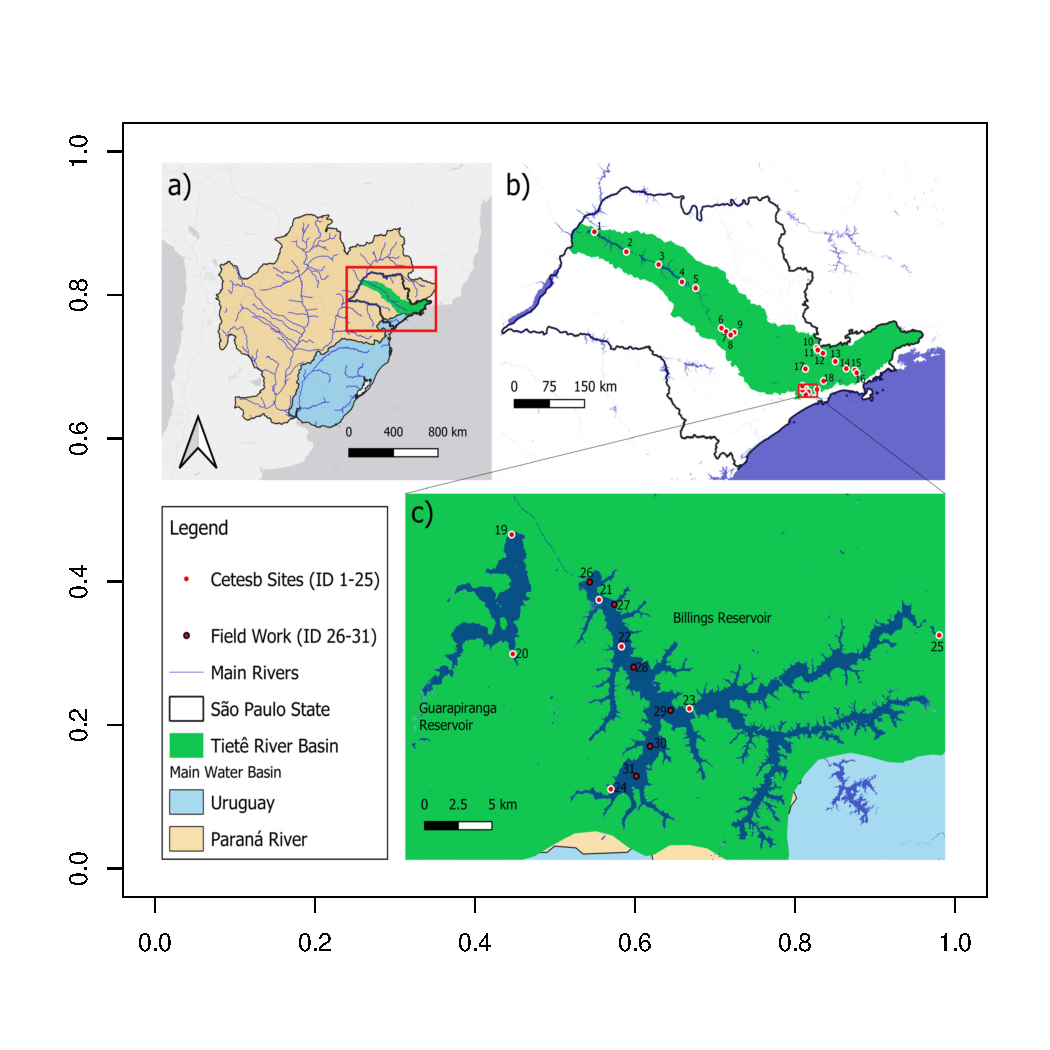
\includegraphics[width=3in,height=\textheight]{spalgae.pdf}

}

\caption{\label{fig-first}(a) Region of Interest is the Paraná River
Water Basin; (b) Tietê River Basin with indication of the sample
stations (see Table 1), (c) Detail of Guarapiranga and Billings
Reservoirs.}

\end{figure}

\hypertarget{tbl-one}{}
\begin{longtable}[]{@{}lllll@{}}
\caption{\label{tbl-one}D-optimality values for design X under five
different scenarios.}\tabularnewline
\toprule\noalign{}
one & two & three & four & five \\
\midrule\noalign{}
\endfirsthead
\toprule\noalign{}
one & two & three & four & five \\
\midrule\noalign{}
\endhead
\bottomrule\noalign{}
\endlastfoot
1.23 & 3.45 & 5.00 & 1.21 & 3.41 \\
1.23 & 3.45 & 5.00 & 1.21 & 3.42 \\
1.23 & 3.45 & 5.00 & 1.21 & 3.43 \\
\end{longtable}

\begin{itemize}
\tightlist
\item
  Note that figures and tables (such as Figure~\ref{fig-first} and
  Table~\ref{tbl-one}) should appear in the paper, not at the end or in
  separate files.
\item
  In document front matter, you may set the key \texttt{blinded} under a
  \texttt{journal} key to hide the authors and acknowledgements,
  producing the required anonymized version.
\item
  Remember that in the anonymized version, you should not identify
  authors indirectly in the text. That is, don't say ``In Smith et.
  al.~(2009) we showed that \ldots{}''. Instead, say ``Smith et.
  al.~(2009) showed that \ldots{}''.
\item
  These points are only intended to remind you of some requirements.
  Please refer to the instructions for authors at
  \url{http://amstat.tandfonline.com/action/authorSubmission?journalCode=uasa20\&page=instructions\#.VFkk7fnF_0c}
\item
  For more about ASA~style, please see
  \url{https://files.taylorandfrancis.com/asa-style-guide.pdf}.
\item
  If you have supplementary material (e.g., software, data, technical
  proofs), identify them in the section below. In early stages of the
  submission process, you may be unsure what to include as supplementary
  material. Don't worry---this is something that can be worked out at
  later stages.
\end{itemize}

\hypertarget{sec-meth}{%
\section{Methods}\label{sec-meth}}

Don't take any of these section titles seriously. They're just for
illustration.

\hypertarget{sec-verify}{%
\section{Verifications}\label{sec-verify}}

This section will be just long enough to illustrate what a full page of
text looks like, for margins and spacing.

\addtolength{\textheight}{.5in}%

\citet{gelm:veht:2021} offer some guidance about key ideas about
statistical ideas. On an unrelated note, spreadsheets are important to
use correctly \citep{brom:woo:2018}. Log-linear models are an attractive
way to model categorical data \citep{bish:fien:1975}.

The quick brown fox jumped over the lazy dog. The quick brown fox jumped
over the lazy dog. The quick brown fox jumped over the lazy dog. The
quick brown fox jumped over the lazy dog. \textbf{With this spacing we
have 25 lines per page.} The quick brown fox jumped over the lazy dog.
The quick brown fox jumped over the lazy dog. The quick brown fox jumped
over the lazy dog. The quick brown fox jumped over the lazy dog. The
quick brown fox jumped over the lazy dog.

The quick brown fox jumped over the lazy dog. The quick brown fox jumped
over the lazy dog. The quick brown fox jumped over the lazy dog. The
quick brown fox jumped over the lazy dog. The quick brown fox jumped
over the lazy dog. The quick brown fox jumped over the lazy dog. The
quick brown fox jumped over the lazy dog. The quick brown fox jumped
over the lazy dog. The quick brown fox jumped over the lazy dog. The
quick brown fox jumped over the lazy dog.

The quick brown fox jumped over the lazy dog. The quick brown fox jumped
over the lazy dog. The quick brown fox jumped over the lazy dog. The
quick brown fox jumped over the lazy dog. The quick brown fox jumped
over the lazy dog. The quick brown fox jumped over the lazy dog. The
quick brown fox jumped over the lazy dog. The quick brown fox jumped
over the lazy dog. The quick brown fox jumped over the lazy dog. The
quick brown fox jumped over the lazy dog.

The quick brown fox jumped over the lazy dog. The quick brown fox jumped
over the lazy dog. The quick brown fox jumped over the lazy dog. The
quick brown fox jumped over the lazy dog. The quick brown fox jumped
over the lazy dog. The quick brown fox jumped over the lazy dog. The
quick brown fox jumped over the lazy dog. The quick brown fox jumped
over the lazy dog. The quick brown fox jumped over the lazy dog. The
quick brown fox jumped over the lazy dog.

\addtolength{\textheight}{-.5in}%

\addtolength{\textheight}{.2in}%

The quick brown fox jumped over the lazy dog. The quick brown fox jumped
over the lazy dog. The quick brown fox jumped over the lazy dog. The
quick brown fox jumped over the lazy dog. The quick brown fox jumped
over the lazy dog. The quick brown fox jumped over the lazy dog. The
quick brown fox jumped over the lazy dog. The quick brown fox jumped
over the lazy dog. The quick brown fox jumped over the lazy dog. The
quick brown fox jumped over the lazy dog.

The quick brown fox jumped over the lazy dog. The quick brown fox jumped
over the lazy dog. The quick brown fox jumped over the lazy dog. The
quick brown fox jumped over the lazy dog. The quick brown fox jumped
over the lazy dog. The quick brown fox jumped over the lazy dog. The
quick brown fox jumped over the lazy dog. The quick brown fox jumped
over the lazy dog. The quick brown fox jumped over the lazy dog. The
quick brown fox jumped over the lazy dog.

The quick brown fox jumped over the lazy dog. The quick brown fox jumped
over the lazy dog. The quick brown fox jumped over the lazy dog. The
quick brown fox jumped over the lazy dog. The quick brown fox jumped
over the lazy dog. The quick brown fox jumped over the lazy dog. The
quick brown fox jumped over the lazy dog. The quick brown fox jumped
over the lazy dog. The quick brown fox jumped over the lazy dog. The
quick brown fox jumped over the lazy dog.

The quick brown fox jumped over the lazy dog. The quick brown fox jumped
over the lazy dog. The quick brown fox jumped over the lazy dog. The
quick brown fox jumped over the lazy dog. The quick brown fox jumped
over the lazy dog. The quick brown fox jumped over the lazy dog. The
quick brown fox jumped over the lazy dog. The quick brown fox jumped
over the lazy dog. The quick brown fox jumped over the lazy dog. The
quick brown fox jumped over the lazy dog.

The quick brown fox jumped over the lazy dog. The quick brown fox jumped
over the lazy dog. The quick brown fox jumped over the lazy dog. The
quick brown fox jumped over the lazy dog. The quick brown fox jumped
over the lazy dog. The quick brown fox jumped over the lazy dog. The
quick brown fox jumped over the lazy dog. The quick brown fox jumped
over the lazy dog. The quick brown fox jumped over the lazy dog. The
quick brown fox jumped over the lazy dog.

The quick brown fox jumped over the lazy dog. The quick brown fox jumped
over the lazy dog. The quick brown fox jumped over the lazy dog. The
quick brown fox jumped over the lazy dog. The quick brown fox jumped
over the lazy dog. The quick brown fox jumped over the lazy dog. The
quick brown fox jumped over the lazy dog. The quick brown fox jumped
over the lazy dog. The quick brown fox jumped over the lazy dog. The
quick brown fox jumped over the lazy dog.

The quick brown fox jumped over the lazy dog. The quick brown fox jumped
over the lazy dog. The quick brown fox jumped over the lazy dog. The
quick brown fox jumped over the lazy dog.

\addtolength{\textheight}{-.2in}%

\hypertarget{sec-conc}{%
\section{Conclusion}\label{sec-conc}}

\hypertarget{disclosure-statement}{%
\section{Disclosure statement}\label{disclosure-statement}}

The authors have the following conflicts of interest to declare (or
replace with a statement that no conflicts of interest exist).

\hypertarget{data-availability-statement}{%
\section{Data Availability
Statement}\label{data-availability-statement}}

Deidentified data have been made available at the following URL: XX.

\hypertarget{supplementary-material}{}
\bigskip

\begin{center}

{\large\bf SUPPLEMENTARY MATERIAL}

\end{center}

\begin{description}
\item[Title:]
Brief description. (file type)
\item[R-package for MYNEW routine:]
R-package MYNEW containing code to perform the diagnostic methods
described in the article. The package also contains all datasets used as
examples in the article. (GNU zipped tar file)
\item[HIV data set:]
Data set used in the illustration of MYNEW method in
Section~\ref{sec-verify} (.txt file).
\end{description}

\hypertarget{bibtex}{%
\section{BibTeX}\label{bibtex}}

We encourage you to use BibTeX. If you have, please feel free to use the
package natbib with any bibliography style you're comfortable with. The
.bst file agsm has been included here for your convenience.


  \bibliography{bibliography.bib}


\end{document}
